\chapter{Introduction}
\label{ch:intro}

Over the past decade deep learning has been reaching unimaginable heights, possibly starting another industrial revolution. Numerous problems were solved with extraordinary accuracies, surpassing previous solutions, as well as human performance. Self-driving cars and automated transportation, digital personal assistants, fraud detection, natural language processing are just some of the tasks whose solutions use deep learning algorithms. But arguably the biggest impact was made in the field of computer vision, with image classification, object detection and segmentation, image colorization, reconstruction, super-resolution and synthesis, and as a result, the entire healthcare industry is on a verge of a major transformation. Deep learning algorithms could be used in various ways, such as analyzing electronic health records, detecting heart problems, diagnosing cancer, planning, navigating and performing surgery.

\section{Medical Image Analysis}

Majority of the data present in medicine (over 90\% of it) belongs to the imaging data, and it is natural to assume that deep learning could have huge impact in the future of medicine. Computed tomography (CT), magnetic resonance imaging (MRI) and X-rays are just some of the medical imaging techniques which produce data that can be used in deep learning algorithms. In this paper I will focus on analysis of histopathology slides, microscopic images of tissue obtained during biopsy.

\section{Histopathologic Cancer Detection}
Histopathologic cancer detection refers to the problem of detecting cancerous tumors in pathologic scans of lymph nodes, organs of the lymphatic system (widely present throughout the body), which act as filters for foreign particles and cancer cells. This task is clinically-relevant, as pathologists analyze a great number of histopathologic slides on a daily basis, which is time-consuming and tedious task prone to misinterpretation. Hence a lucrative solution would reduce their workload, speed up the process, and improve the prediction accuracy. In this paper, I propose a deep learning algorithm to solve this task.

\section{Datasets}
Digital pathology is field in medical imaging, where whole-slide scanners are used to digitize glass slides containing tissue at high resolution, in order to be viewed, managed, shared and analyzed on a computer. The advance of digital pathology has led to the high availability of digital images, which has in turn led to creation of datasets on which deep learning methods can be applied. In this paper, I will train neural networks on two such datasets, BreakHis and NCT-CRC-HE-100K dataset.

\subsection{BreakHis Dataset}

The Breast Cancer Histopathological Image Classification\cite{breakhis_article} (BreakHis) is a dataset constructed in collaboration with Pathological Anatomy and Cytopathology Laboratory (Parana, Brazil) which contains 9.109 images of breast tumor tissue. It is collected from 82 patients, using different magnifying factors (40x, 100x, 200x, and 400x), and contains 2.480  benign and 5.429 malignant samples (700x460 pixels). Dataset is divided into two main groups, benign tumors (do not invade nearby tissue or spread to other parts of the body) and malignant tumors (can invade nearby tissues, made of cancer cells). Based on the way cells look under the microscope, there are eight subtypes of tumors: adenosis, fibroadenoma, phyllodes tumors and tubular adenona for benign tumors, and carcinoma, lobular carcinoma, mucinous carcinoma and papillary carcinoma for malignant tumors (\textcolor{red}{\autoref{fig:breakhis}}).

\captionsetup[figure]{font=scriptsize,labelfont=scriptsize}

\begin{figure}[h]
	\centering
	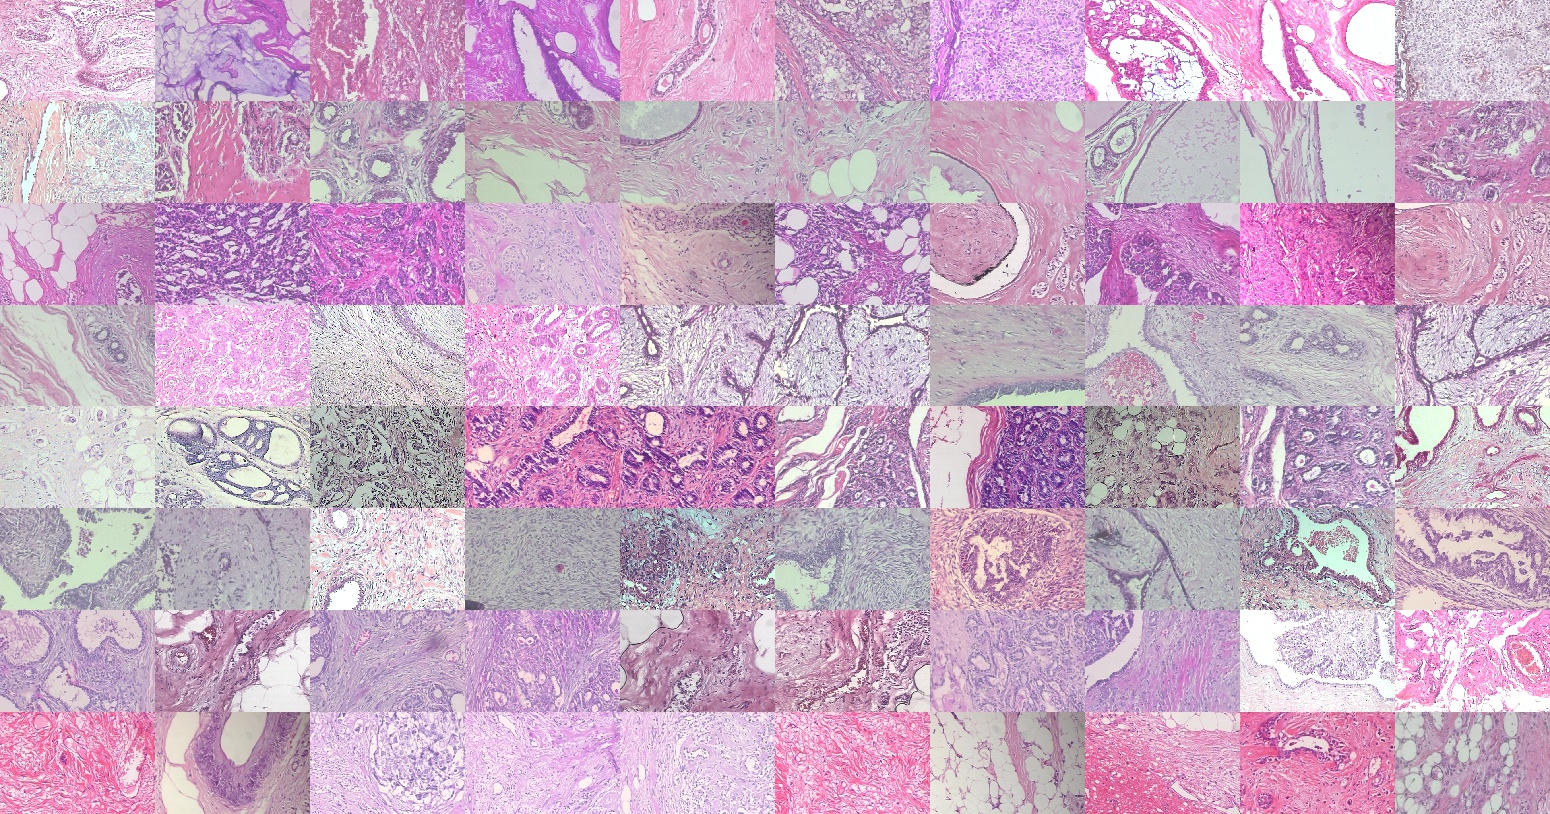
\includegraphics[scale=0.32]{break_his_dataset.jpg}
	\caption{BreakHis dataset tissue classes: adenosis, ductal carcinoma, fibroadenoma, lobular carcinoma, mucinous carcinoma, papillary carcinoma, phyllodes tumor, tubular adenoma}
	\label{fig:breakhis}
\end{figure}

\subsection{NCT-CRC-HE-100K Dataset}

The NCT-CRC-HE-100K is a dataset constructed in collaboration with National Center for Tumor diseases (Heidelberg, Germany) which contains 100.000 images of colorectal tumor tissue. It is collected from 86 patients, using 100x magnifying factor (224x224 pixels). Based on the way cells look under the microscope, there are nine subtypes of tissue: adipose, background, debris, lymphocytes, mucus, smooth muscle, normal colon mucosa, cancer-associated stroma and colorectal adenocarcinoma epithelium (\textcolor{red}{\autoref{fig:nctcrche100k}}).

\begin{figure}[h]
	\centering
	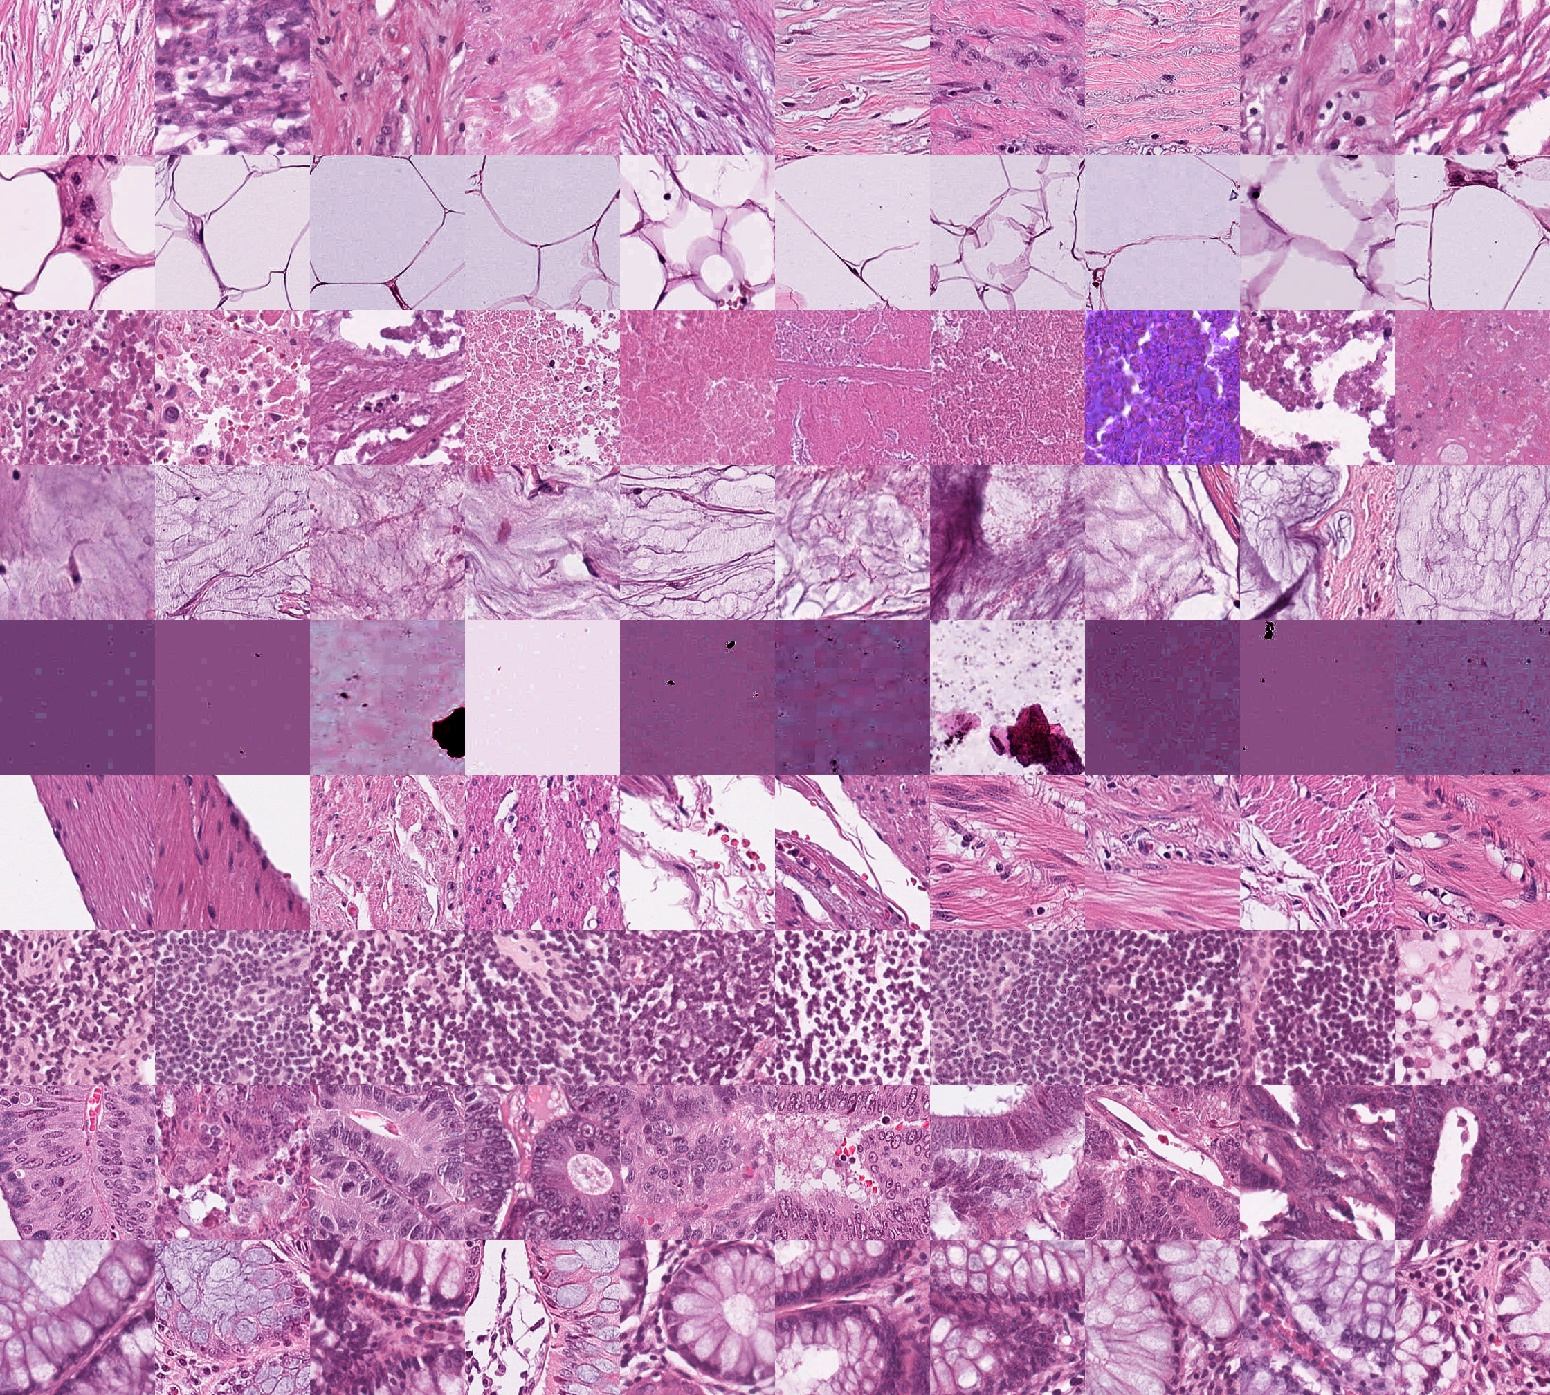
\includegraphics[scale=0.22]{nct_crc_he_100k_dataset.jpg}
	\caption{NCT-CRC-HE-100K dataset tissue classes: adipose tissue, background, debris, lymphocytes, mucus, smooth muscle, normal colon mucosa, cancer-associated stroma, colorectal adenocarcinoma epithelium}
	\label{fig:nctcrche100k}
\end{figure}

\section{Approach}

I have divided the creation of the program for histopathologic cancer detection in four major parts:
\begin{enumerate}
	\itemsep0em
	\item Assembling dataset structure (required for input to convolutional neural network), image preprocessing (loading, removing noise, normalization, whitening) and data augmentation (expanding size of dataset by applying a series of random transformations to each image)
	\item Building the convolutional neural networks (class of deep neural networks applied to analyzing images), and training them on data
	\item Improving prediction accuracy of networks (solving underfitting and overfitting problems) with hyperparameter tuning (choosing optimal parameters for learning algorithm) and changes to network architecture
	\item Creating graphical user interface for the program, which allows user to load histopathologic slide and select network which has be applied on it, and to get as output category to which that slide belongs, with additional possibility to visualize network representations (heatmaps of class activations, filters of convolutional layers and intermediate activations)
\end{enumerate}
